\documentclass[12pt]{article}
\textwidth=17cm \oddsidemargin=-0.9cm \evensidemargin=-0.9cm
\textheight=23.7cm \topmargin=-1.7cm

\usepackage{amssymb, amsmath, amsfonts}
\usepackage{moreverb}
\usepackage{graphicx}
\usepackage{enumerate}
\usepackage{graphics}
\usepackage{color}
\usepackage{array}
\usepackage{float}
\usepackage{hyperref}
\usepackage{textcomp}
\usepackage{alltt}
\usepackage{physics}
\usepackage{mathtools}
\usepackage{tikz}
\usetikzlibrary{positioning}
\usetikzlibrary{arrows}
\usepackage{pgfplots}
\usepackage{bigints}
\usepackage[utf8]{inputenc}
\usepackage[english]{babel}
\usepackage{amsthm}
\usepackage{fancyhdr}
\usepackage[makeroom]{cancel}
\pagestyle{fancy}
\allowdisplaybreaks

\newcommand{\E}{\varepsilon}

\newcommand{\suchthat}{\, \mid \,}
\newcommand{\ol}[1]{\overline{#1}}
\newcommand{\bbar}[1]{\overline{#1}}
\newcommand{\inpd}[1]{{\left< \, #1 \, \right>}}
\renewcommand{\theenumi}{\alph{enumi}}
\newcommand\Wider[2][3em]{%
\makebox[\linewidth][c]{%
  \begin{minipage}{\dimexpr\textwidth+#1\relax}
  \raggedright#2
  \end{minipage}%
  }%
}

\def\R{\mathbb{R}}
\def\C{\mathbb{C}}
\def\H{\mathcal{H}}
\DeclareMathOperator*{\esssup}{\text{ess~sup}}
\newcommand{\resolv}[1]{\rho(#1)}
\newcommand{\spec}[1]{\sigma(#1)}
\newcommand{\iffR}{\noindent \underline{$\Longrightarrow$:} }
\newcommand{\iffL}{\noindent \underline{$\Longleftarrow$:} }
\newcommand{\lightning}{\textbf{\Huge \Lightning}}
\newcommand{\spt}[1]{\text{spt}(#1)}
\def\ran{\text{ ran}}
   
\newenvironment{myprob}[1]
    {%before text commands
    %{\Huge \_ \_ \_ \_ \_ \_ \_ \_ \_ \_ \_ \_ \_ \_ \_ \_ \_ \_ } \\
    \noindent{\Huge$\ulcorner$}\textbf{#1.}\begin{em}
    }
    { 
    %after text commands
    \end{em} \\ \hphantom{l} \hfill {\Huge$\lrcorner$} }
%	{\noindent \rule{7.5cm}{2pt} \textgoth{#1} \rule{8.cm}{2pt} \begin{em}}
%	{\end{em}\\ \vspace{0.1pt}\noindent \rule{\textwidth}{2pt}}
%
\setcounter{section}{-1}




\begin{document}
\lhead{MATH228A}
\chead{Carter Johnson - Homework 02}
\rhead{\today}

{\let\newpage\relax} 


%%%%%%%%%%%%%%%%%%%%%%%%%%%%%%%%%%%%%%%%%%%%%%%%%%%%% P1
\begin{myprob}{Problem 1}
Use the standard 3-point discretization of the Laplacian on a regular mesh to find a numerical
solution to the PDEs below. Perform a refinement study using the exact solution to compute
the error that shows the rate of convergence for both the 1-norm and the max norm.
\end{myprob}
%%%%%%%%%%%%%%% part a
\begin{enumerate}[ \ \ (a)]
\item $u_{xx} = e^{x}$, $u(0)=0$, $u(1)=1$
\end{enumerate}
We can compute the solution to this PDE analytically:
\begin{align*}
u_{xx} &= e^{x}\\
u_x &= e^{x} + c_1 \\
u &= e^{x} +c_1 x + c_2 \\
u(0)=0 &= e^{0} + 0 + c_2 \implies c_2 = -1 \\
u(1) = 1 &= e^{1} + c_1 -1 \implies c_1 = 2-e\\
\implies u(x) &= e^{x} + (2-e)x -1 .
\end{align*}
We then solve the PDE numerically for various grid spacings $h$ and grid points $x_1, \dots x_N$ (where $N=1/h - 1$), with each trial using the standard 3-point discretization of the Laplacian
 \begin{align*}
            A = \frac{1}{h^2}\qty(\begin{array}{ccccc}
                -2 & 1 & & & \\
                1 & -2 & 1 & \\
                & & \ddots & & \\
                & & 1 & -2 & 1 \\
                & & & 1 & -2
            \end{array})
  \end{align*}
and discretizing the RHS of the PDE, including the BC's
        \begin{align*}
            \vec{b} = \qty(\begin{array}{c}
                f_1 - \frac{0}{h^2} \\ f_2 \\ \vdots \\ f_{N-1} \\ f_N - \frac{1}{h^2}
            \end{array}).
        \end{align*}
For each $h$, we solve the linear system $A\vec{u} = \vec{b}$ for $\vec{u}$, and calculate the error in both the 1-norm and the max-norm compared to our analytic solution evaluated at the same grid points.  The refinement study is as follows:
\begin{figure}[H]
\centering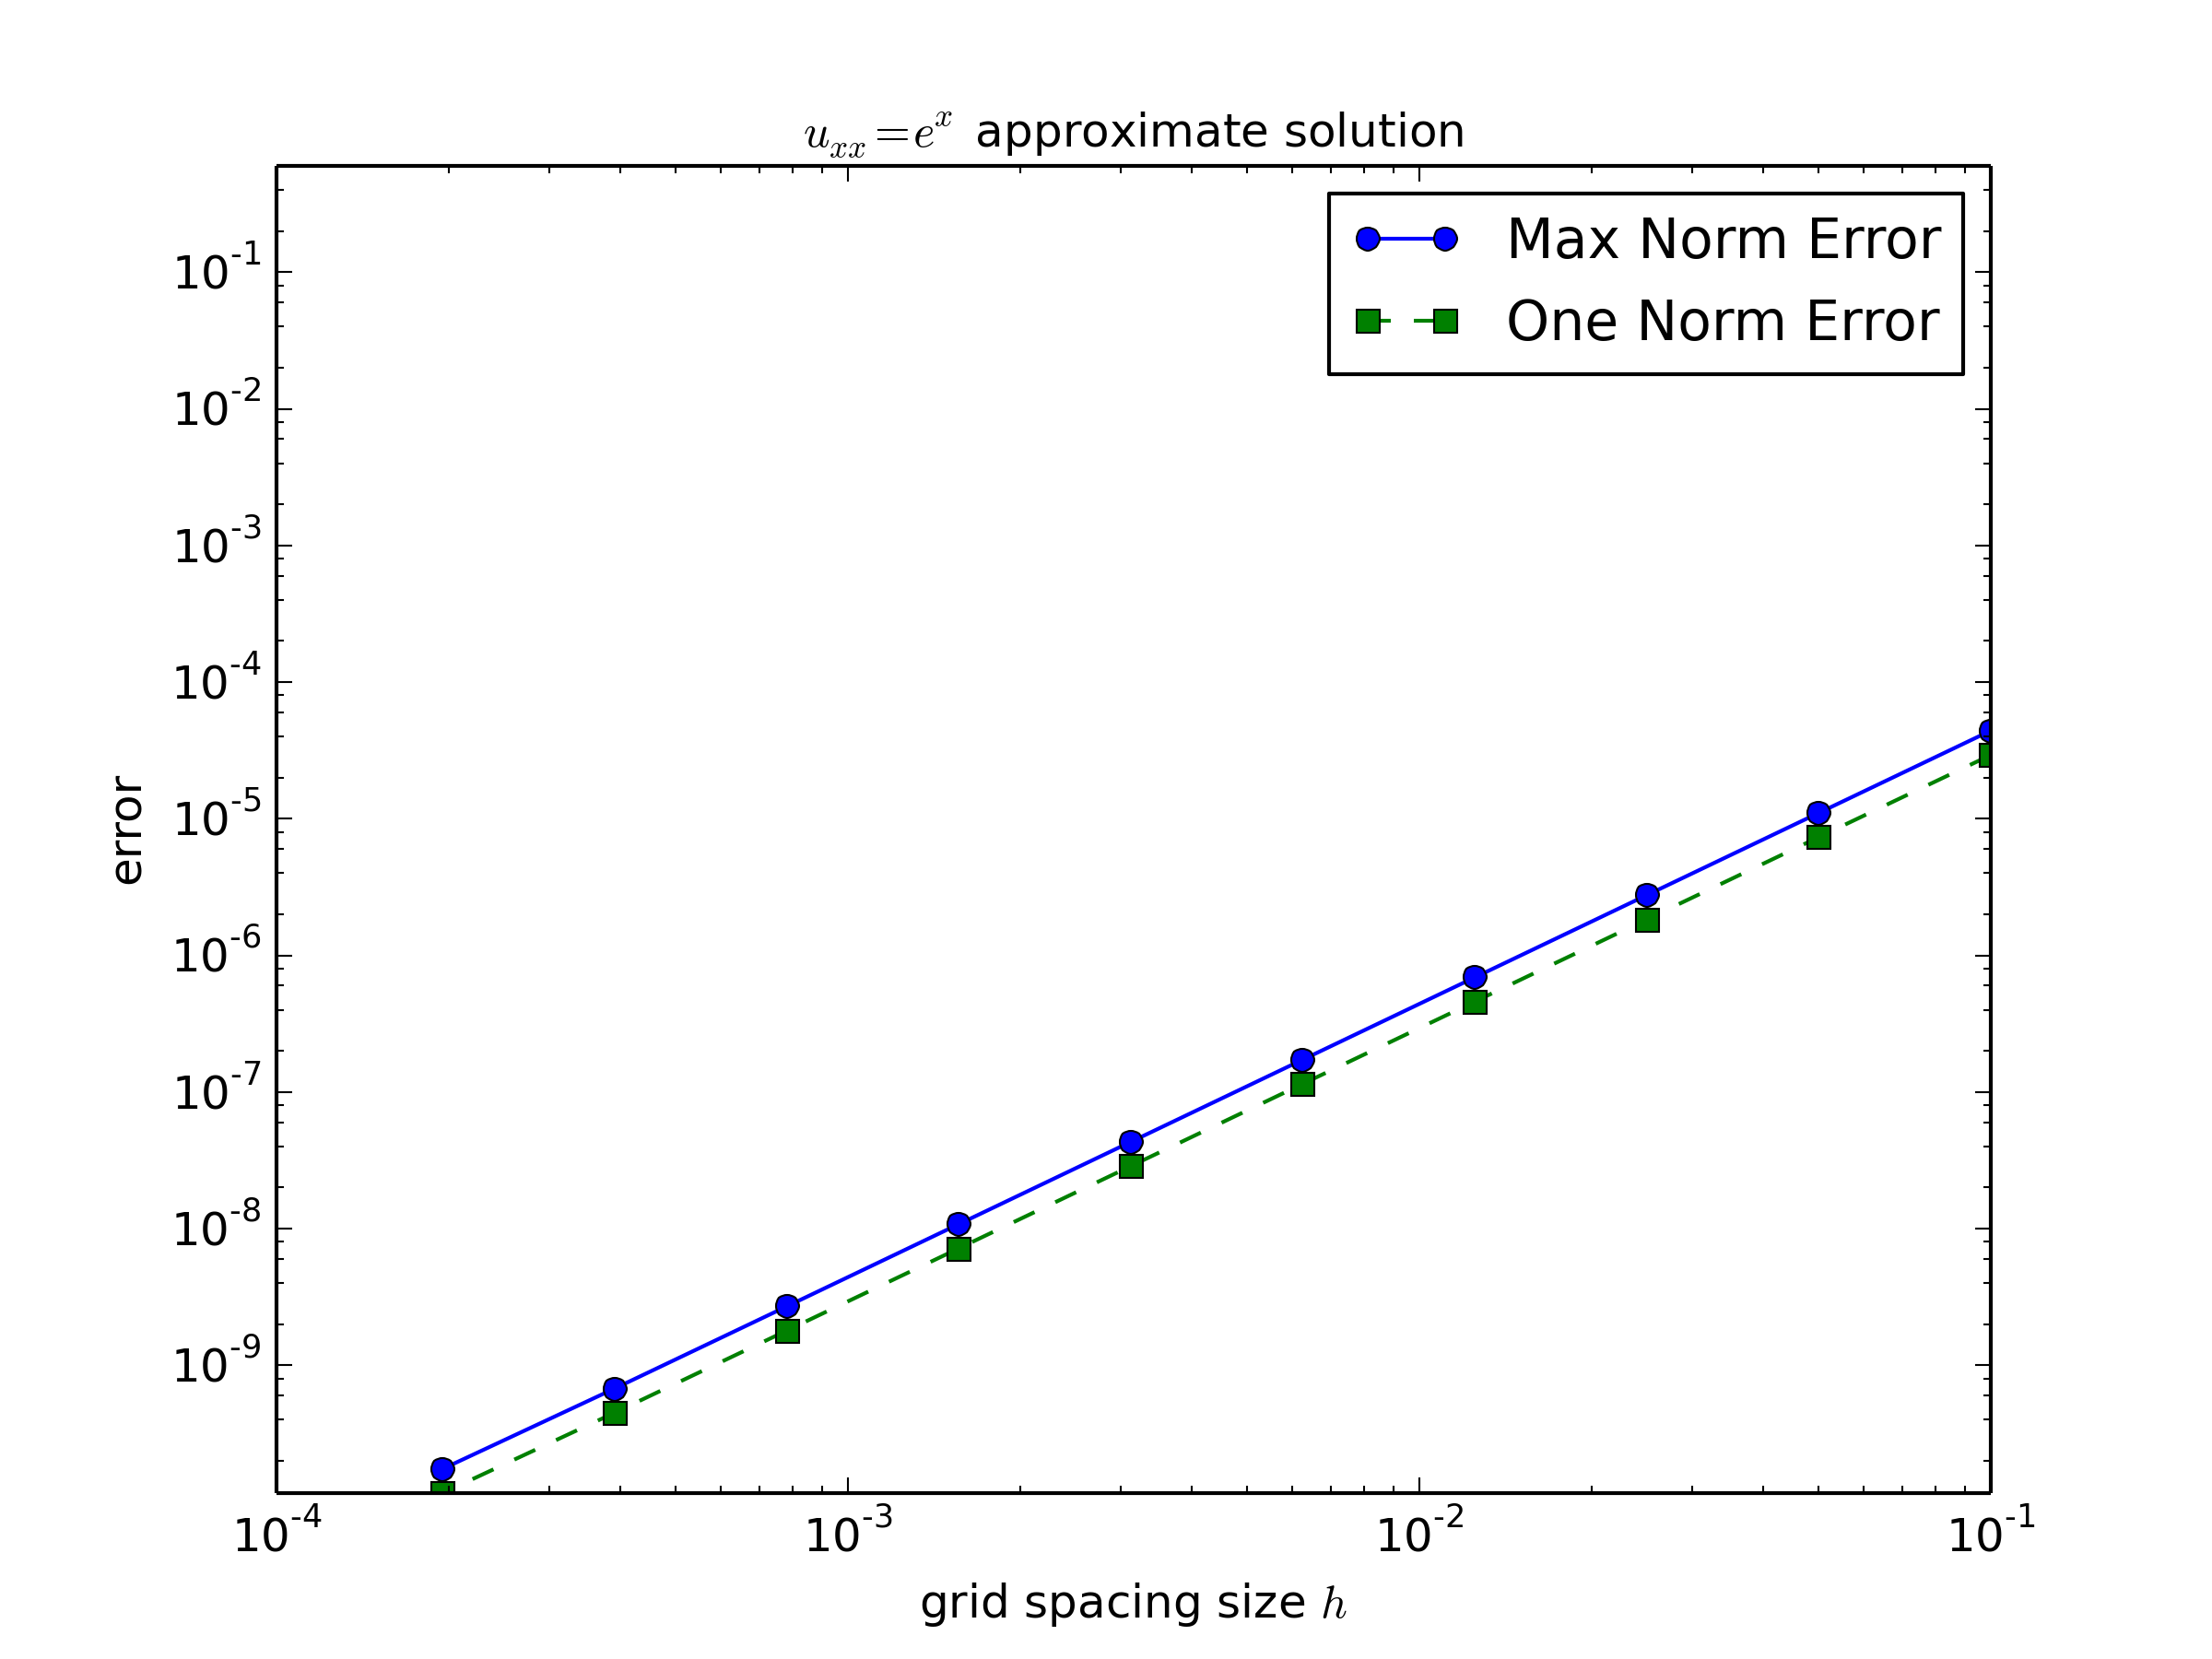
\includegraphics[scale=0.5]{problem1a_refinement_study.png}
\caption{The refinement study for the numerical solution of the PDE $u_{xx} = e^{x}$ for various grid sizes $h$, compared to the analytic solution in the one-norm and the max-norm. Note that we have convergence in both the max-norm and the one-norm, though the one-norm converges faster.}
\end{figure}

\begin{center}
\begin{tabular}{rrr}
\hline
Grid Spacing Size &  One-Norm Error & Successive Error Ratio \\
\hline
 0.1         & 2.92674e-05 & 0.250501 \\
 0.05        & 7.33152e-06 & 0.250125 \\
 0.025       & 1.8338e-06  & 0.250031 \\
 0.0125      & 4.58507e-07 & 0.250008 \\
 0.00625     & 1.1463e-07  & 0.250002 \\
 0.003125    & 2.86577e-08 & 0.249997 \\
 0.0015625   & 7.16434e-09 & 0.25     \\
 0.00078125  & 1.79109e-09 & 0.250826 \\
 0.000390625 & 4.49252e-10 & 0.258063 \\
\hline
\end{tabular}\\
\begin{tabular}{rrr}
\hline
Grid Spacing Size &  Max-Norm Error & Successive Error Ratio \\
\hline
 0.1         & 4.41199e-05 & 0.250023 \\
 0.05        & 1.1031e-05  & 0.250068 \\
 0.025       & 2.7585e-06  & 0.25001  \\
 0.0125      & 6.89653e-07 & 0.250006 \\
 0.00625     & 1.72417e-07 & 0.25     \\
 0.003125    & 4.31042e-08 & 0.249997 \\
 0.0015625   & 1.07759e-08 & 0.250003 \\
 0.00078125  & 2.69401e-09 & 0.250788 \\
 0.000390625 & 6.75626e-10 & 0.258043 \\
\hline
\end{tabular}
\end{center}

From the refinement study, it is clear that as we halve the grid spacing size, the error in both the one and max norms are quartered, so the solution is converging like $\order{h^2}$.
\newpage

%%%%%%%%%%%%%%% part b
\begin{enumerate}[ \ \ (b)]
\item $u_{xx} = 2\cos^2(\pi x)$, $u_x(0)=0$, $u_x(1)=1$
\end{enumerate}
We first ensure that this PDE is solvable:
\begin{align*}
\int_0^1 u_{xx} \ \dd x &= \int_0^1 2 \cos^2(\pi x) \ \dd x \\
u_x(1) - u_x(0) &= \int_0^1 1 + \cos(2 \pi x) \ \dd x \\
1 &= \qty[x + \dfrac{1}{2\pi}\sin(2 \pi x)]_0^1 = 1.
\end{align*} 
The PDE is in fact solvable, but it does not have a unique solution since the operator $u_{xx}$ (with homogeneous Neumann BC's) has a nullspace spanned by $u = 1$.  Our discrete Laplacian (with inhomogeneous Neumann BC's) problem has the form

 \begin{align*}
             \frac{1}{h^2}\qty(\begin{array}{ccccc}
                -1 & 1 & & & \\
                1 & -2 & 1  & & \\
                & 1 & -2 & 1  \\
                & & \ddots & & \\
                & & 1 & -2 & 1 \\
                & & & 1 & -1
            \end{array})
            \qty(\begin{array}{c}
            u_0 \\
            u_1 \\
            \vdots \\
            \vdots \\
            u_N \\
            u_{N+1}
            \end{array})
            = \qty(\begin{array}{c}
            f_0/2 + 0/h \\
            f_1 \\
            \vdots \\
            \vdots \\
            f_N \\
            f_{N+1}/2 - 1/h
            \end{array}).
  \end{align*}
The discrete Laplacian operator $A$ has a nullspace spanned by 
        \begin{align*}
            \vec{v} = \qty(\begin{array}{c}
                1 \\ 1 \\ \vdots \\ 1 \\ 1
            \end{array}) = \vec{1}.
        \end{align*}
Then in order for our corresponding discretization of the RHS to yield a solution to $A\vec{u} = \vec{b}$, we must have that $\vec{b} \in \ran{A} = (\ker{A})^\perp$, i.e., $\vec{b} \cdot \vec{1} = 0$.  If not, then we can project $b$ onto the range 
$$\vec{b}_{\text{proj}} = \vec{b} - \qty(\dfrac{\vec{1}\cdot\vec{b}}{\vec{1}\cdot\vec{1}})\vec{1} = \vec{b} - \lambda \vec{v},$$ and solve the projected equation $$Au = \vec{b}_{\text{proj}}.$$
We also need to pick a unique solution to our PDE, so we pick the one with mean zero, i.e., $\vec{1} \cdot \vec{u} = 0$.  Thus we have to solve the augmented system
 \begin{align*}
A\vec{u} + \lambda \vec{1} &= \vec{b} \\
\vec{1} \cdot \vec{u} &= 0
 \end{align*}
 using the augmented block matrix form $A_{aug} (\vec{u}, \lambda) = (\vec{b}, 0)$.

The analytic solution can be easily obtained
\begin{align*}
u_{xx} &= 1 + \cos(2\pi x) \\
u_x &= x + \dfrac{1}{2\pi} \sin(2 \pi x) + c_1 \\
u_x(0) &= 0 = c_1 \implies c_1 =0 \\
\implies u &= \dfrac{x^2}{2} - \dfrac{1}{4\pi^2} \cos(2 \pi x) + c
\end{align*}
where $c$ is some constant, so this solution is unique up to an additive constant.  Note that $u_x(1) = 1 + 0 = 1$, so this does indeed solve the Neumann problem.

For each $h$, we solve the linear system $A_{aug} (\vec{u}, \lambda) = (\vec{b}, 0)$ for $\vec{u}$, and calculate the error in both the 1-norm and the max-norm compared to our analytic solution evaluated at the same grid points.  To pick the particular analytic solution to compare to, we choose the analytic solution whose discretization wrt. $h$ has zero mean, i.e., we pick $c$ s.t. $\vec{1} \cdot (u(0), u(x_1), \dots, u(x_N), u(1)) = 0$.  This yields 
$$u(x_i) = \dfrac{x_i^2}{2} - \dfrac{1}{4\pi^2} \cos(2\pi x_i) - \dfrac{\sum_{j=0}^{N+1} \dfrac{x_j^2}{2} - \dfrac{1}{4\pi^2} \cos(2 \pi x_j)}{N+2}$$
The refinement study is as follows:
\begin{figure}[H]
\centering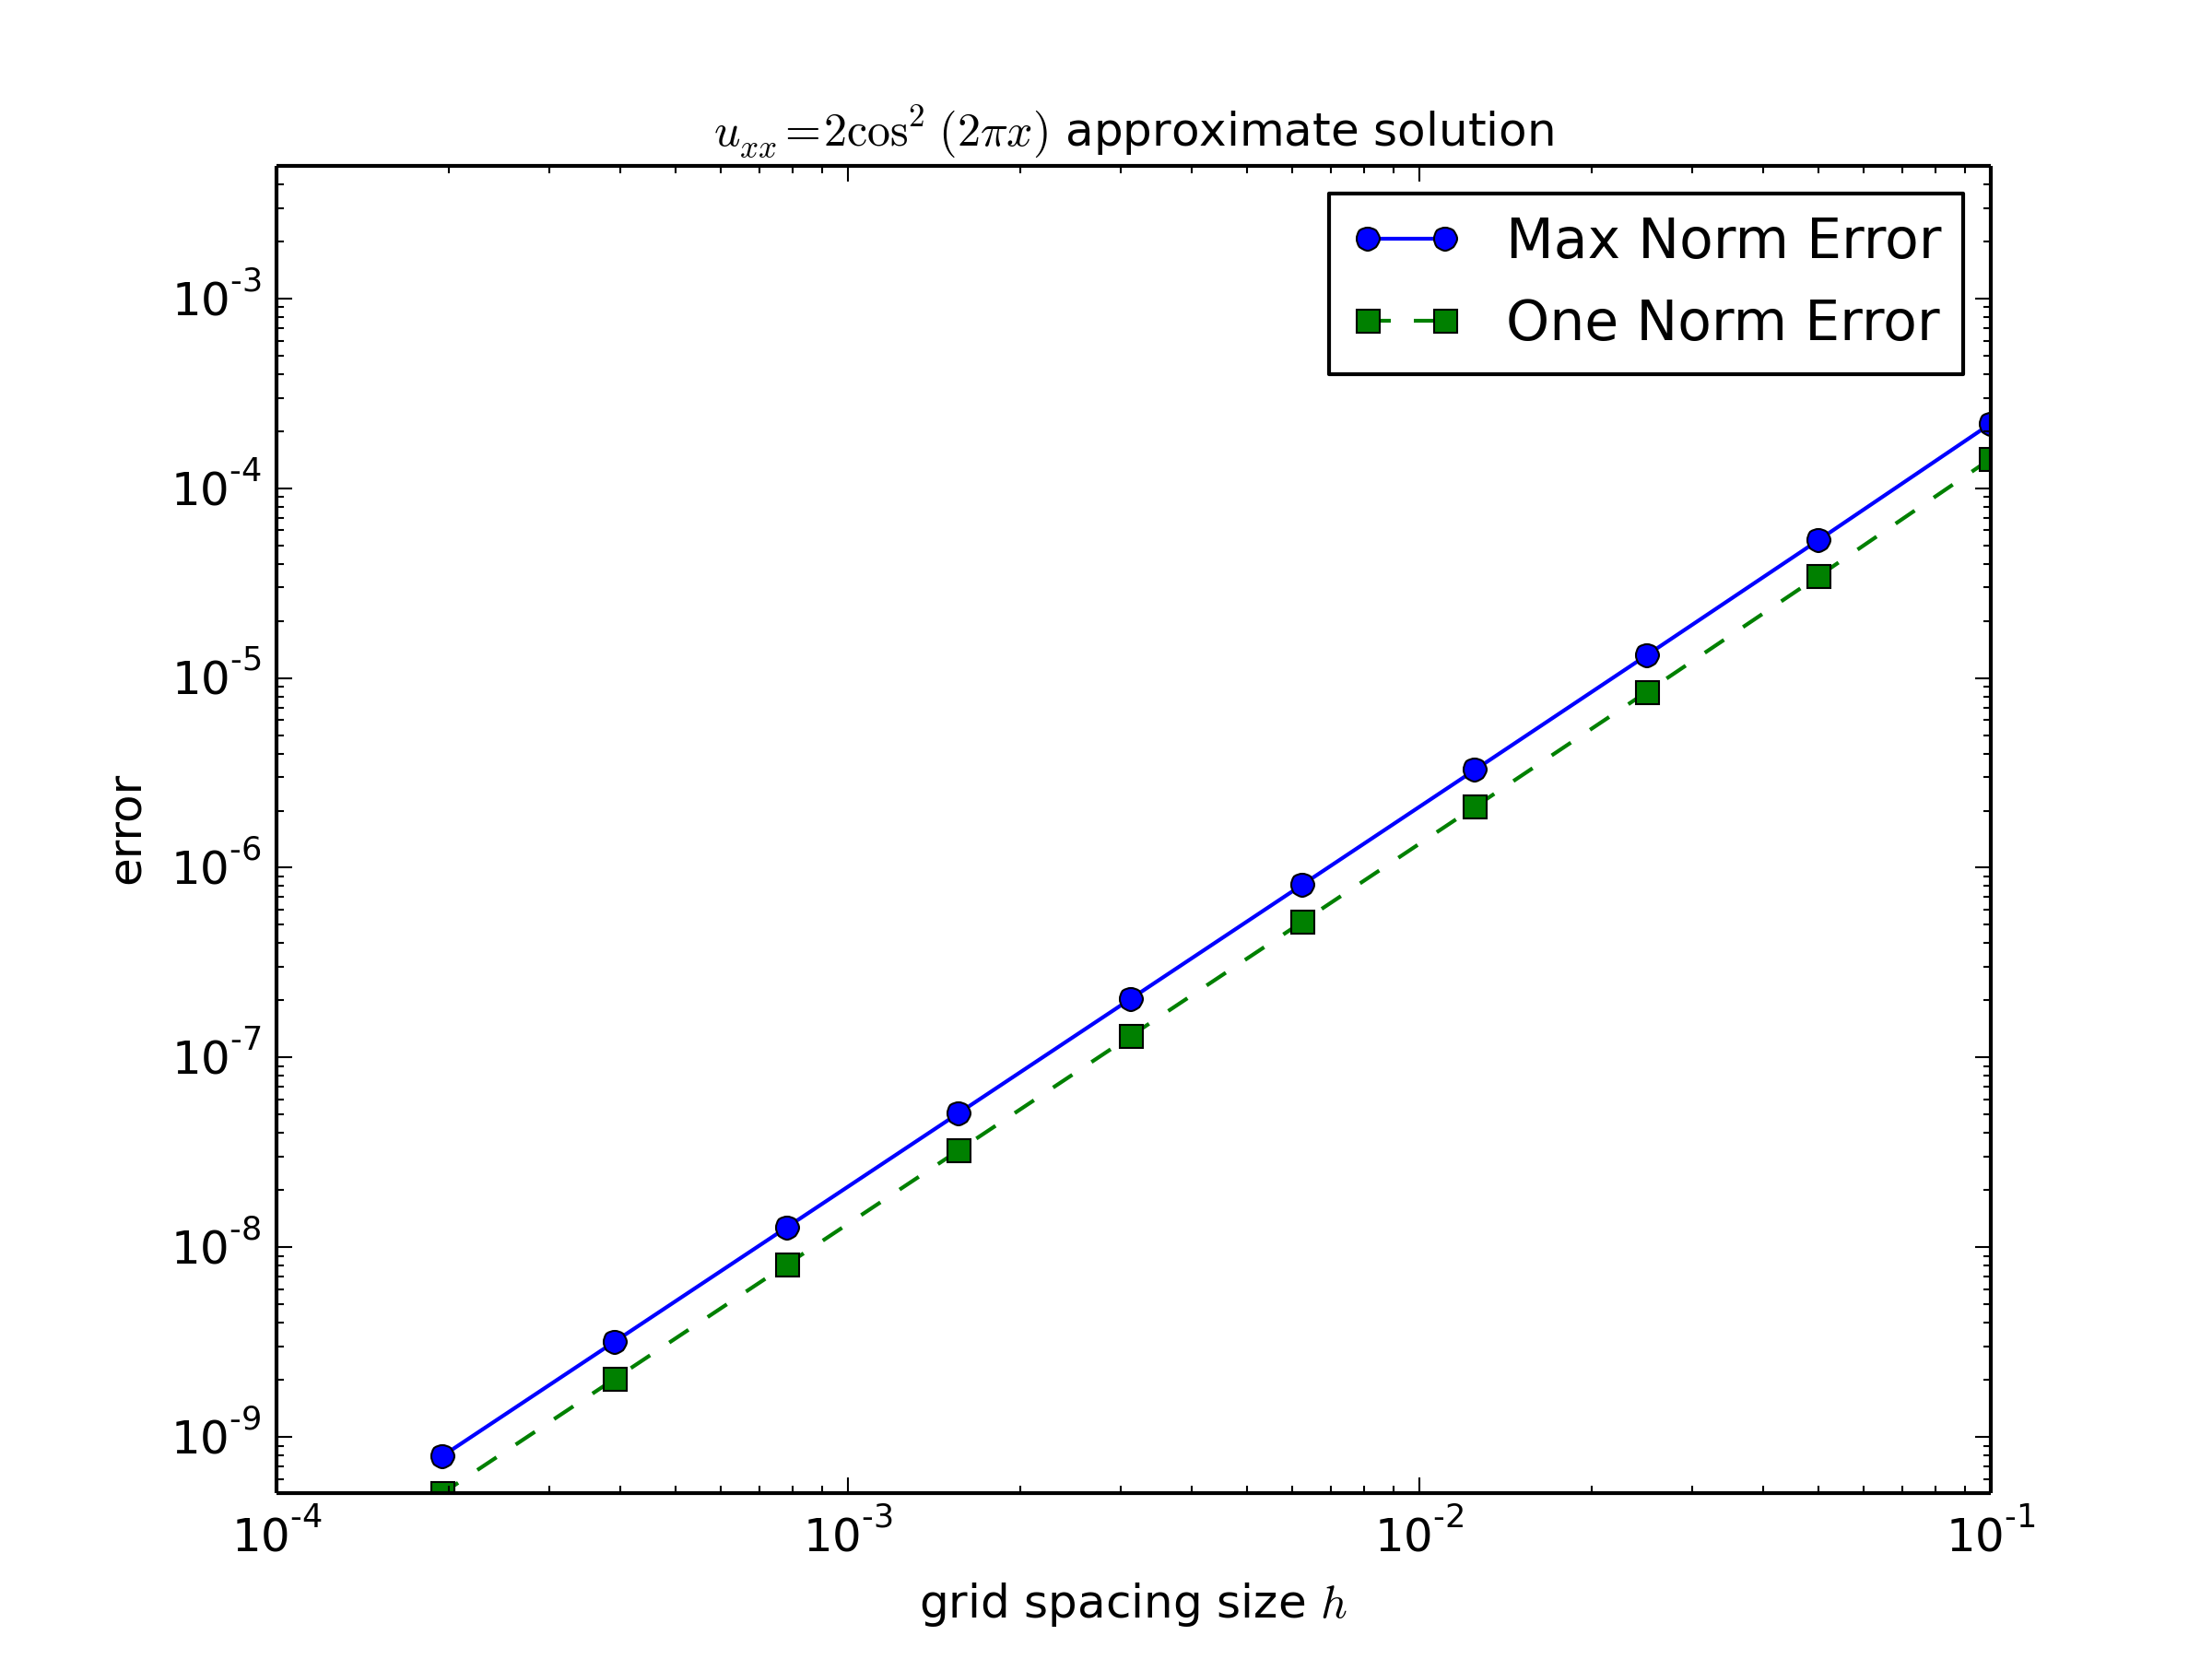
\includegraphics[scale=0.5]{problem1b_refinement_study.png}
\caption{The refinement study for the numerical solution of the PDE $u_{xx} = 2\cos^2(\pi x)$ for various grid sizes $h$, compared to the analytic solution in the one-norm and the max-norm. Note that we have convergence in both the max-norm and the one-norm, though the one-norm converges slightly faster.}
\end{figure}

\begin{center}
\begin{tabular}{rrr}
\hline
Grid Spacing Size &  One-Norm Error & Successive Error Ratio \\
\hline
 0.1         & 0.000143155 & 0.240756 \\
 0.05        & 3.44654e-05 & 0.245244 \\
 0.025       & 8.45244e-06 & 0.247585 \\
 0.0125      & 2.0927e-06  & 0.248783 \\
 0.00625     & 5.20627e-07 & 0.249389 \\
 0.003125    & 1.29839e-07 & 0.249694 \\
 0.0015625   & 3.24199e-08 & 0.249847 \\
 0.00078125  & 8.10001e-09 & 0.249923 \\
 0.000390625 & 2.02438e-09 & 0.249962 \\
\hline
\end{tabular}\\
\begin{tabular}{rrr}
\hline
Grid Spacing Size &  Max-Norm Error & Successive Error Ratio \\
\hline
 0.1         & 0.000219335 & 0.243552 \\
 0.05        & 5.34195e-05 & 0.246832 \\
 0.025       & 1.31857e-05 & 0.248428 \\
 0.0125      & 3.27568e-06 & 0.249216 \\
 0.00625     & 8.16353e-07 & 0.249609 \\
 0.003125    & 2.03769e-07 & 0.249805 \\
 0.0015625   & 5.09024e-08 & 0.249902 \\
 0.00078125  & 1.27206e-08 & 0.24995  \\
 0.000390625 & 3.17952e-09 & 0.249968 \\
\hline
\end{tabular}
\end{center}


From the refinement study, it is clear that as we halve the grid spacing size, the error in both the one and max norms are almost quartered, so the solution is converging like $\order{h^2}$.\\

%%%%%%%%%%%%%%%%%%%%%%%%%%%%%%%%%%%%%%%%%%%%%%%%%%%%% P1
\begin{myprob}{Problem 2}
As a general rule, we usually think that an $\order{h^p}$ local truncation error (LTE) leads to an $\order{h^p}$ error. However, in some cases the LTE can be lower order at some points without lowering the order of the error.  Consider the standard second-order discretization of the Poisson equation on $[0,1]$ with homogenous boundary conditions.  The standard discretization of this problem gives an $\order{h^2}$ LTE provided the solution is at least $C^4$.  The LTE may be lower order because the solution is not $C^4$ or because we use a lower order discretization at some points.
\end{myprob}
%%%%%%%%%%%%%%% part a
\begin{enumerate}[(a)]
\item Suppose that the LTE is $\order{h^p}$ at the first grid point $(x_1 = h)$. What effect does this have on the error? What is the smallest value of $p$ that gives a second order accurate error?  Hint: Use equation (2.46) from LeVeque to aid in your argument.
\end{enumerate}

The total error $\vec{e}$ of our discretization $A \vec{u} = \vec{f}$
is given by $A\vec{e} = -\vec{\tau}$, where $\vec{\tau}$ is the LTE.  If $\vec{\tau}_1 = \order{h^p}$ and $\vec{\tau}_i = \order{h^2}$ for $i=2,\dots, n$, then using the inverse $A^{-1}= B$ where $$B_{ij} = h(x_> - 1)x_< \ \ \text{ (with }x_> = x_j, x_< = x_i \text{ for }j\geq i)$$ we have
$$ \vec{e} = -B \vec{\tau} = -\sum_{j=1}^n \vec{b_j} \tau_j.$$

\noindent Note that for an interior point $x_j$, $\tau_j = \order{h^2}$ and
\begin{align*}
\vec{b_j} = \qty(\begin{array}{c}
              h(x_j - 1)x_1 \\
               \vdots \\
               h(x_j - 1)x_{j-1} \\
               h(x_j - 1)x_{j} \\
               h(x_{j+1} - 1)x_{j} \\
               \vdots \\
               h(x_n - 1)x_j   
            \end{array})
\end{align*}
so the largest element of $\vec{b_j}$ is the $j^{th}$, $B_{jj} = h(x_j - 1)x_j  = \order{h}$ since $x_j$ by definition is an interior point which does not go to the boundary as $h\to0$, i.e., $x_j = \order{1}$.  Thus $$\vec{b_j}\tau_j = \order{h} \order{h^2} = \order{h^3}.$$

\noindent But for the boundary point $x_1$, $\vec{b_1}$ has largest element $B_{11} = h(x_1 -1)x_1 = h(h-1)h = \order{h^2}$,
so $$\vec{b_1}\tau_1 = \order{h^{p+2}}.$$
So for $p= 0$, $\vec{b_1}\tau_1 = \order{h^2}$, and for $p>0$, $\vec{b_1}\tau_1 = o(h^2)$.
Hence if $p \geq 0$, this LTE has no effect on the total error, as 
$$-\vec{e} = \sum_{j=1}^n \vec{b_j}\tau_j = o(h^2) + \sum_{j=2}^n \order{h^3} = \order{h^2}$$
since we sum up $n-1 = \order{1/h}$ terms.
On the other hand, if $p<0$ then $\vec{b_1}\tau_1$ will be lower-order than $\order{h^2}$, so it will dominate the total error, so $\vec{e} = \order{h^{p+2}}$.  The smallest value of $p$ that gives a second-order accurate error is $p=0$.
%%%%%%%%%%%%%%% part b
\begin{enumerate}[(b)]
\item Suppose that the LTE is $\order{h^p}$ at an interior point (i.e., a point that does not limit to the boundary as $h\to0$). What effect does this have on the error? What is the smallest value of $p$ that gives a second order accurate error?
\end{enumerate}

Let the LTE $\tau_i = \order{h^p}$ for some interior point $x_i$. Then
\begin{align*}
\vec{b_i} = \qty(\begin{array}{c}
              h(x_i - 1)x_1 \\
               \vdots \\
               h(x_i - 1)x_{i-1} \\
               h(x_i - 1)x_{i} \\
               h(x_{i+1} - 1)x_{i} \\
               \vdots \\
               h(x_n - 1)x_i   
            \end{array}),
\end{align*}
so the largest element of $\vec{b_i}$ is the $i^{th}$, $B_{ii} = h(x_i - 1)x_i  = \order{h}$ since $x_i$ by definition is an interior point which does not go to the boundary as $h\to0$, i.e., $x_j = \order{1}$.  Thus $$\vec{b_i}\tau_i = \order{h} \order{h^p} = \order{h^{p+1}},$$ while the other $\vec{b_j}\tau_j$ remain $\order{h^3}$ (or smaller for the points near the boundary).   Then 
$$-\vec{e}=\sum_{j=1}^n \vec{b_j}\tau_j = \vec{b_i}\tau_i + \sum_{j=1, j\neq i}^n \order{h^3}= \order{h^{p+1}} + \order{h^2}.$$  Hence to get a second-order accurate approximation, we require that $p\geq 1$.

%%%%%%%%%%%%%%% part c
\begin{enumerate}[ \ \ (c)]
\item Verify the results of your analysis from parts (a) and (b) using numerical tests.
\end{enumerate}
Local truncation error is given by $$\vec{\tau} = A\vec{u} - \vec{b}.$$
To verify the analysis from parts (a) and (b), we will modify the code from question 1 part (a).  
The LTE at a boundary point $x_j$ in that problem is given by
$$\tau_j = \dfrac{1}{h^2}(u(x_{j-1}) -2u(x_j) + u(x_{j+1})) -f(x_j) = u_{xx}(x_j) + \dfrac{h^2}{2}u^{(4)}(x_j) + \text{h.o.t.} - f(x_j) = \order{h^2}.$$
To make the LTE $\order{h^p}$ here instead, we can simply perturb $f(x_j)$ by $\order{h^p}$, so let $$f^p(x_j) = f(x_j) + h^p.$$
Then we will modify the code to use $f^p(x_j)$ instead of $f(x_j)$ for the boundary point $x_1 = h$.

Running the refinement study from 1a, we have that for $p=-1$:\\
\begin{center}
\begin{tabular}{rrr}
\hline
    h &  1-norm Error &   Succesive Error Ratio \\
\hline
 0.1         &                   0.0237207   &                0.513482 \\
 0.05        &                   0.0121802   &                0.506565 \\
 0.025       &                   0.00617004  &                0.50324  \\
 0.0125      &                   0.00310501  &                0.501609 \\
 0.00625     &                   0.0015575   &                0.500802 \\
 0.003125    &                   0.000780001 &                0.5004   \\
 0.0015625   &                   0.000390313 &                0.5002   \\
 0.00078125  &                   0.000195234 &                0.5001   \\
 0.000390625 &                   9.76367e-05 &                0.50005  \\
\hline
\end{tabular}
\end{center}
So the $\order{h^{-1}}$ LTE at the boundary made the total error $\order{h}$.
For $p=0$:\\
\begin{center}
\begin{tabular}{rrr}
\hline
    h &   1-norm Error &   Succesive Error Ratio \\
\hline
 0.1         &                   0.00115823  &                0.256733 \\
 0.05        &                   0.000297356 &                0.253281 \\
 0.025       &                   7.53146e-05 &                0.25162  \\
 0.0125      &                   1.89507e-05 &                0.250805 \\
 0.00625     &                   4.75292e-06 &                0.250401 \\
 0.003125    &                   1.19014e-06 &                0.2502   \\
 0.0015625   &                   2.97773e-07 &                0.2501   \\
 0.00078125  &                   7.44731e-08 &                0.25003  \\
 0.000390625 &                   1.86205e-08 &                0.24983  \\
\hline
\end{tabular} 
\end{center}
So the $\order{1}$ LTE at the boundary left the total error $\order{h^2}$.  Hence $p=0$ is indeed the minimum needed for second-order accuracy.  For $p=1$: \\
\begin{center}
\begin{tabular}{rrr}
\hline
    h &   1-norm Error &   Succesive Error Ratio \\
\hline
 0.1         &                   3.29023e-05 &                0.139734 \\
 0.05        &                   4.59758e-06 &                0.263404 \\
 0.025       &                   1.21102e-06 &                0.297113 \\
 0.0125      &                   3.59811e-07 &                0.280355 \\
 0.00625     &                   1.00875e-07 &                0.266129 \\
 0.003125    &                   2.68457e-08 &                0.258214 \\
 0.0015625   &                   6.93192e-09 &                0.254138 \\
 0.00078125  &                   1.76166e-09 &                0.252914 \\
 0.000390625 &                   4.4555e-10  &                0.259162 \\
\hline
\end{tabular}
\end{center}
So the $\order{h}$ LTE at the boundary indeed also gives $\order{h^2}$ total accuracy.
The LTE at an interior point $x_j$ in that problem is given by
$$\tau_j = \dfrac{1}{h^2}(u(x_{j-1}) -2u(x_j) + u(x_{j+1})) -f(x_j) = u_{xx}(x_j) + \dfrac{h^2}{2}u^{(4)}(x_j) + \text{h.o.t.} - f(x_j) = \order{h^2}.$$
To make the LTE $\order{h^p}$ here instead, we can simply perturb $f(x_j)$ by $\order{h^p}$, so let $$f^p(x_j) = f(x_j) + h^p.$$
Then we will modify the code to use $f^p(x_j)$ instead of $f(x_j)$ for the fixed interior point $x_{N/2} = 1/2$.
Running the refinement study from 1a, we have that for $p=0$:
\begin{center}
\begin{tabular}{rrr}
\hline
    h &   1-norm Error &   Succesive Error Ratio \\
\hline
 0.1         &                   0.00622073  &                0.501174 \\
 0.05        &                   0.00311767  &                0.500588 \\
 0.025       &                   0.00156067  &                0.500294 \\
 0.0125      &                   0.000780791 &                0.500147 \\
 0.00625     &                   0.00039051  &                0.500073 \\
 0.003125    &                   0.000195284 &                0.500037 \\
 0.0015625   &                   9.76491e-05 &                0.500018 \\
 0.00078125  &                   4.88263e-05 &                0.500009 \\
 0.000390625 &                   2.44136e-05 &                0.500004 \\
\hline
\end{tabular}
\end{center}
So the $\order{1}$ LTE at the interior point $x_{N/2} = 1/2$ gives $\order{h}$ total error.  For $p=1$:
\begin{center}
\begin{tabular}{rrr}
\hline
    h &   Interior Point 1-norm Error &   Succesive Error Ratio \\
\hline
 0.1         &                   0.000283233 &                0.249948 \\
 0.05        &                   7.07935e-05 &                0.249987 \\
 0.025       &                   1.76975e-05 &                0.249997 \\
 0.0125      &                   4.42431e-06 &                0.249999 \\
 0.00625     &                   1.10607e-06 &                0.25     \\
 0.003125    &                   2.76518e-07 &                0.25     \\
 0.0015625   &                   6.91296e-08 &                0.25     \\
 0.00078125  &                   1.72824e-08 &                0.249914 \\
 0.000390625 &                   4.31912e-09 &                0.249161 \\
\hline
\end{tabular}
\end{center}
So the $\order{h}$ LTE at the interior point gives $\order{h^2}$ accuracy, so $p=1$ is indeed the minimum necessary for second-order accuracy.
For $p=2$: \\
\begin{center}
\begin{tabular}{rrr}
\hline
    h &   1-norm Error &   Succesive Error Ratio \\
\hline
 0.1         &                   1.36424e-05 &                0.394241 \\
 0.05        &                   5.3784e-06  &                0.295563 \\
 0.025       &                   1.58966e-06 &                0.269234 \\
 0.0125      &                   4.27989e-07 &                0.258921 \\
 0.00625     &                   1.10816e-07 &                0.254305 \\
 0.003125    &                   2.81809e-08 &                0.252112 \\
 0.0015625   &                   7.10474e-09 &                0.251049 \\
 0.00078125  &                   1.78364e-09 &                0.251351 \\
 0.000390625 &                   4.48319e-10 &                0.258344 \\
\hline
\end{tabular}
\end{center}
So the $\order{h^2}$ LTE at an interior point indeed also gives $\order{h^2}$ total accuracy. \\

%%%%%%%%%%%%%%%%%%%%%%%%%%%%%%%%%%%%%%%%%%%%%%%%%%%%% P3
\begin{myprob}{Problem 3}
We have typically discretized the interval $[0,1]$ into equally spaced points $x_j = jh$ for $j=0, \dots, N+1$ with $h=1/(N+1)$.  Another common discretization is the cell centered mesh, in which $[0,1]$ is discretized into $N$ cells. This approach is commonly used with finite-volume methods.  The grid points are placed at centers of the cells: $x_j = (j-1/2)h$ for $j=1, \dots , N$ where $h=1/N$.  This type of discretization is more natural for some problems, particularly those with Neumann boundary conditions.
\end{myprob}
%%%%%%%%%%%%%%% part a
\begin{enumerate}[ \ \ (a)]
\item We may write $u_{xx} = (-J)_x$, where $J=-u_x$ is the diffusive flux.  Suppose we discretize this problem by using a centered difference to compute the flux at the cell edges, $J_{j-1/2} = -u_x((j-1)h)$, followed by another centered difference of the flux.  Show that at interior points, this gives the standard second-order discretization of $u_{xx}$.  
\end{enumerate}

We will approximate $u_{xx}(x_j)$ for an interior point $x_j = (j-1/2)h$.
With a centered difference approximation,
$$J_{j-1/2} = -u_x((j-1)h) \approx \dfrac{u(x_{j-1})-u(x_j)}{h} = \dfrac{u((j-3/2)h) - u((j-1/2)h)}{h}, $$
and $$J_{j+1/2} = -u_x(jh) \approx \dfrac{u(x_{j})-u(x_{j+1})}{h} = \dfrac{u((j-1/2)h) - u((j+1/2)h)}{h}. $$
So with another centered difference, 
\begin{align*}
u_{xx}((j-1/2)h)= u_{xx}(x_j) = (-J_j)_x &\approx \dfrac{J_{j-1/2} - J_{j+1/2}}{h} = \dfrac{u(x_{j-1})-2u(x_j)+u(x_{j+1})}{h^2} \\
&= \dfrac{u((j-3/2)h) - 2u((j-1/2)h) + u((j+1/2)h)}{h^2}.
\end{align*}
Note this is the standard second-order discretization of $u_{xx}$.

%%%%%%%%%%%%%%% part b
\begin{enumerate}[ \ \ (b)]
\item Again using the idea of flux differencing, derive the discrete approximation to $u_{xx}$ at the first interior grid point adjacent to a boundary with Neumann boundary condition $u_x = g$.
\end{enumerate}

We will approximate $u_{xx}(x_1) = u_{xx}(h/2)$ for the first interior grid point at $x_1 = h/2$.
Using the centered difference as in (a), 
$$u_{xx}(x_1) \approx \dfrac{J_{1-1/2} - J_{1+1/2}}{h}.$$
Now since $J_{1-1/2}=J_{1/2}$ is the negative flux across the boundary at $x=0$, $J_{1/2} = - g$ by our Neumann condition.  We use the centered difference approximation for $J_{1+1/2}$ as in (a) to obtain
$$u_{xx}(x_1) \approx \dfrac{-g - \qty(\dfrac{u(x_1)-u(x_2)}{h})}{h} = \dfrac{-gh -u(x_1)+u(x_2)}{h}.$$
%%%%%%%%%%%%%%% part c
\begin{enumerate}[ \ \ (c)]
\item The cell-centered discretization seems awkward for Dirichlet boundary conditions because the spacing from the boundary to the first interior grid point is not equal to the spacing between interior grid points.  One option for discretizing the second derivative at the first interior point is to use the finite difference stencil we derived in the first homework assignment.  Alternately, a common discretization of $u_{xx}$ at $x_1$ with given boundary value $u(0)$ is
$$\dfrac{2u(0)-3u(x_1) + u(x_2)}{h^2} = f_1.$$
What is the local truncation error of this discretization?  What order of accuracy do you expect for the numerical solution?
\end{enumerate}

To find the local truncation error, we look at the Taylor series centered at $x_1$ for each term in the discretization.
$$u(0) = u(x_1 - h/2) = u(x_1) - \dfrac{h}{2}u'(x_1) + \dfrac{h^2}{8}u''(x_1) - \dfrac{h^3}{48}u'''(x_1) + \dots$$
$$u(x_2) = u(x_1 + h) = u(x_1) + hu'(x_1) + \dfrac{h^2}{2}u''(x_1) + \dfrac{h^3}{6}u'''(x_1) + \dots$$
So $$\dfrac{2u(0)-3u(x_1) + u(x_2)}{h^2} = \dfrac{3h^2/4  u''(x_1) + \order{h^3}}{h^2} = \dfrac{3}{4} u''(x_1) + \order{h},$$
which is an $\order{1}$ accurate approximation of $u''(x_1)$.  Thus the LTE of $u_{xx}$ at $x_1$ is $\order{1}=\order{h^0}$, which still allows for second-order accuracy in the full approximation as per problem 2 part a.

%%%%%%%%%%%%%%%%%%%%%%%%%%%%%%%%% done
\noindent\rule{17cm}{0.4pt}

\noindent \textbf{Python Code used for 1a:}
\begin{verbatim}
#MAT228A Homework 2
#Question 1, Part A

#Use standard 3-pt Lapacian discretization 
#to find soluton to u_xx = exp(x), u(0)=0, u(1)=1

#perform a refinement study using exact solution
#to show error convergence for 1-norm and max 1-norm

from __future__ import division

import numpy as np
from math import exp

import matplotlib.pyplot as plt
import scipy.sparse as sparse
import scipy.sparse.linalg
import tabulate

#Refinement study loop size
max_loop = 10

#initialize grid size vector, error vectors
h=1/10
grid_spacing_size = [h/(2**i) for i in range(max_loop)]
one_norm_errors = np.zeros(max_loop)
max_norm_errors = np.zeros(max_loop)


#Loop for refinement study
for i in range(max_loop):

  #size of grid spacing
  h = h/2
  #Set number of grid points
  N = 1/h - 1

  #set grid points starting from h to 1-h 
  #since we include Dirichlet conditions in RHS
  x = np.linspace(h, 1-h, num=N)
  #set RHS of PDE, Au(x_i) = f(x_i) = b
  b = np.exp(x)
  #include BC u(1)=1 in RHS, (u(0)=0 trivially included)
  b[-1] = b[-1] - 1/(h**2)

  #set sparse matrix A, the discrete Laplacian
  offdiag = (1/(h**2))*np.ones(N)
  diag = np.ones(N)*(-2/(h**2))
  data = np.vstack((offdiag, diag,offdiag))
  A = sparse.dia_matrix((data, [-1, 0,1]), shape = (N,N))
  A_CSC_form = scipy.sparse.csc_matrix(A)

  #solve Au = b
  approx_u = scipy.sparse.linalg.spsolve(A_CSC_form, b)

  #find actual solution u(x) = e^x + (2-e)x -1
  u = np.exp(x) + (2-exp(1))*x - np.ones(N)

  #one norm error
  one_norm_errors[i] = h*np.sum(np.abs(u-approx_u))

  #max norm error
  max_norm_errors[i] = np.amax(np.abs(u-approx_u))

#give table of ratios of successive errors
one_norm_table = [[grid_spacing_size[i], one_norm_errors[i], one_norm_errors[i+1]/one_norm_errors[i]] for i in range(max_loop-1)]
print tabulate.tabulate(one_norm_table, headers = ["a", "b", "c"], tablefmt="latex")

max_norm_table = [[grid_spacing_size[i], max_norm_errors[i], max_norm_errors[i+1]/max_norm_errors[i]] for i in range(max_loop-1)]
print tabulate.tabulate(max_norm_table, headers = ["a", "b", "c"], tablefmt="latex")

#plot errors
plt.figure()
plt.loglog(grid_spacing_size, max_norm_errors, '-o', label="Max Norm Error")
plt.loglog(grid_spacing_size, one_norm_errors, '--s', label="One Norm Error")
plt.legend(loc=0)
plt.title(r"$u_{xx} = e^{x}$ approximate solution", fontsize=12)
plt.xlabel(r"grid spacing size $h$")
plt.ylabel("error")
plt.savefig("problem1a_refinement_study.png", dpi=300)
\end{verbatim}\\

\noindent \textbf{Python Code used for 1b:}
\begin{verbatim}
#MAT228A Homework 2
#Question 1, Part B

#Use standard 3-pt Lapacian discretization 
#to find soluton to u_xx = 2cos^2(pi x), u'(0)=0, u'(1)=1

#perform a refinement study using exact solution
#to show error convergence for 1-norm and max 1-norm

from __future__ import division

import numpy as np
from math import exp, pi

import matplotlib.pyplot as plt
import scipy.sparse as sparse
import scipy.sparse.linalg
from scipy.sparse import coo_matrix, bmat
import tabulate

#Refinement study loop size
max_loop = 10

#initialize grid size vector, error vectors
h=1/10
grid_spacing_size = [h/(2**i) for i in range(max_loop)]
one_norm_errors = np.zeros(max_loop)
max_norm_errors = np.zeros(max_loop)

#Loop for refinement study
for i in range(max_loop):

  #size of grid spacing
  h = h/2
  #Set number of grid points
  N = 1/h - 1
  #set grid points
  x = np.linspace(0, 1, num=(N+2))
  #set RHS of PDE, Au(x_i) = f(x_i) = b
  b = 2*(np.cos(pi*x)**2)
  #include BCs u'(0)=0, u'(1)=1 in RHS
  b[0] = b[0]/2 + 0/h
  b[N+1] = b[N+1]/2-1/h

  #set sparse matrix A, the discrete Laplacian
  offdiag = (1/(h**2))*np.ones(N+2)
  diag = np.concatenate(([-1],-2*np.ones(N),[-1]))*(1/(h**2))
  data = np.vstack((offdiag, diag,offdiag))
  A = sparse.dia_matrix((data, [-1, 0,1]), shape = (N+2,N+2))


  #set augmented system matrix for Au + Lambda v = b, 1T u = 0
  A_temp = scipy.sparse.hstack([A, np.ones((N+2,1))])
  A_aug = scipy.sparse.vstack([A_temp, np.concatenate((np.ones(N+2), [0]))
  ])
  A_aug_CSC_form = scipy.sparse.csc_matrix(A_aug)

  #solve Au + Lambda v = b, 1T u = 0
  approx_u = scipy.sparse.linalg.spsolve(A_aug_CSC_form, np.concatenate((b, [0])))
  approx_lambda = approx_u[N+2]
  #get rid of lambda element
  approx_u = np.delete(approx_u, N+2) 
  
  #find actual solution u(x) = x^2/2 - 1/(4pi^2) cos(2pi x) + c
  u = (1/2)*x**2 - 1/(4*pi**2)*np.cos(2*pi*x) - np.sum((1/2)*x**2 - 1/(4*pi**2)*np.cos(2*pi*x))/(N+2)
  
  #one norm error
  one_norm_errors[i] = h*np.sum(np.abs(u-approx_u))

  #max norm error
  max_norm_errors[i] = np.amax(np.abs(u-approx_u))

#give table of ratios of successive errors
one_norm_table = [[grid_spacing_size[i], one_norm_errors[i], one_norm_errors[i+1]/one_norm_errors[i]] for i in range(max_loop-1)]
print tabulate.tabulate(one_norm_table, headers = ["a", "b", "c"], tablefmt="latex")

max_norm_table = [[grid_spacing_size[i], max_norm_errors[i], max_norm_errors[i+1]/max_norm_errors[i]] for i in range(max_loop-1)]
print tabulate.tabulate(max_norm_table, headers = ["a", "b", "c"], tablefmt="latex")

#plot errors
plt.figure()
plt.loglog(grid_spacing_size, max_norm_errors, '-o', label="Max Norm Error")
plt.loglog(grid_spacing_size, one_norm_errors, '--s', label="One Norm Error")
plt.legend(loc=0)
plt.title(r"$u_{xx} = 2\cos^2(2\pi x)$ approximate solution", fontsize=12)
plt.xlabel(r"grid spacing size $h$")
plt.ylabel("error")
plt.savefig("problem1b_refinement_study.png", dpi=300)
\end{verbatim}
\noindent \textbf{Python Code used for 2c:}
\begin{verbatim}
#MAT228A Homework 2
#Question 2, Part C

#Investigate the effect of O(h^p) LTE at interior and boundary points
#on whether the solution to the
#standard 3-pt Lapacian discretization 
#of u_xx = exp(x), u(0)=0, u(1)=1
#changes the order of accuracy


from __future__ import division

import numpy as np
from math import exp

import matplotlib.pyplot as plt
import scipy.sparse as sparse
import scipy.sparse.linalg
import tabulate



#Refinement study loop size
max_loop = 10

#O(h^p) LTE  - vector of orders p
p_orders = [-3, -2, -1, 0, 1, 2, 3] 
p_size = np.size(p_orders)

#initialize grid size vector, error vectors
h=1/10
grid_spacing_size = [h/(2**i) for i in range(max_loop)]
one_norm_errors_pa = np.zeros((max_loop, p_size))
one_norm_errors_pb = np.zeros((max_loop, p_size))


#Loop for refinement study
for i in range(max_loop):

  #size of grid spacing
  h = h/2
  #Set number of grid points
  N = 1/h - 1

  #set grid points starting from h to 1-h 
  #since we include Dirichlet conditions in RHS
  x = np.linspace(h, 1-h, num=N)

  #set sparse matrix A, the discrete Laplacian
  offdiag = (1/(h**2))*np.ones(N)
  diag = np.ones(N)*(-2/(h**2))
  data = np.vstack((offdiag, diag,offdiag))
  A = sparse.dia_matrix((data, [-1, 0,1]), shape = (N,N))
  A_CSC_form = scipy.sparse.csc_matrix(A)

  #find actual solution u(x) = e^x + (2-e)x -1
  u = np.exp(x) + (2-exp(1))*x - np.ones(N)
  
  #Loop for LTE order effects 
  for j in range(p_size):
    
    #Do two analyses:
    #set RHS of PDE, Au(x_i) = f(x_i) = b_pa
    b_pa = np.exp(x)
    #include BC u(1)=1 in RHS, (u(0)=0 trivially included)
    b_pa[-1] = b_pa[-1] - 1/(h**2)
    #include O(h^p) LTE at boundary point x_1=h as in part a
    b_pa[0] = b_pa[0] + (h**p_orders[j])

    #set RHS of PDE, Au(x_i) = f(x_i) = b_pb
    b_pb = np.exp(x)
    #include BC u(1)=1 in RHS, (u(0)=0 trivially included)
    b_pb[-1] = b_pb[-1] - 1/(h**2)
    #include O(h^p) LTE at fixed interior point at x=1/2 as in part b
    b_pb[N/2] = b_pb[N/2] + (h**p_orders[j])

    #solve Au = b for parts a and b
    approx_u_pa = scipy.sparse.linalg.spsolve(A_CSC_form, b_pa)
    approx_u_pb = scipy.sparse.linalg.spsolve(A_CSC_form, b_pb)

    #one norm errors
    one_norm_errors_pa[i,j] = h*np.sum(np.abs(u-approx_u_pa))
    one_norm_errors_pb[i,j] = h*np.sum(np.abs(u-approx_u_pb))



#give tables of ratios of successive errors with given LTE O(h^p)
for j in range(p_size):
  print(p_orders[j])
  one_norm_table_pa = [[grid_spacing_size[i], one_norm_errors_pa[i,j], one_norm_errors_pa[i+1,j]/one_norm_errors_pa[i,j]] for i in range(max_loop-1)]
  print tabulate.tabulate(one_norm_table_pa, headers = ["h", "Boundary Point 1-norm Error", "Succesive Error Ratio"], tablefmt="latex")
  one_norm_table_pb = [[grid_spacing_size[i], one_norm_errors_pb[i,j], one_norm_errors_pb[i+1,j]/one_norm_errors_pb[i,j]] for i in range(max_loop-1)]
  print tabulate.tabulate(one_norm_table_pb, headers = ["h", "Interior Point 1-norm Error", "Succesive Error Ratio"], tablefmt="latex")
\end{verbatim}
%%%%%%%%%%%%%%%%%%%%%%%%%%%%%%%%%%%%%%%%%%%%% end
\end{document}